\documentclass{beamer}
%\mode<presentation>
\usepackage[utf8]{inputenc}
\usepackage[magyar]{babel}
\usetheme{CambridgeUS}
\usecolortheme{dolphin}
\usepackage{amsmath,amssymb,amsfonts}
\usepackage{mathpazo}
\usepackage{graphicx,tabularx,epsfig}
\usepackage{subcaption}
\DeclareGraphicsExtensions{.pdf,.png,.jpg,.svg}



\title{A $v_n$ harmonikusok nehézion-ütközésekben}
\author{Bagoly Attila}
\date[\today]{Kísérleti mag- és részecskefizikai szeminárium\\ \today}
\institute{ELTE TTK}
\begin{document}

\begin{frame}
  \titlepage
\end{frame}

\begin{frame}
\frametitle{Tartalomjegyzék}
\tableofcontents
\end{frame}

\section{Bevezető}
\begin{frame}
\begin{itemize}
\item Célunk: természet alapvető működésének megismerése
\item Ma már tudjuk, hogy a minket körülvevő világ atomokból épül fel
\item Jelenlegi tudásunk szerint minden felépíthető kvarkokból, leptonokból, bozonokból
\item Kvarkok színtöltéssel rendelkeznek, erős kölcsönhatás ezek közt hat
\item Erős kölcsönhatást a kvantum-színdinamika írja le, ez egy ${\rm SU}(3)$ szimmetriájú kvantumtérelmélet
\item QCD: kvarkbezártság és aszimptotikus szabadság (kvark-gluon plazma)
\item Ősrobbanás
\end{itemize}
\end{frame}

\begin{frame}
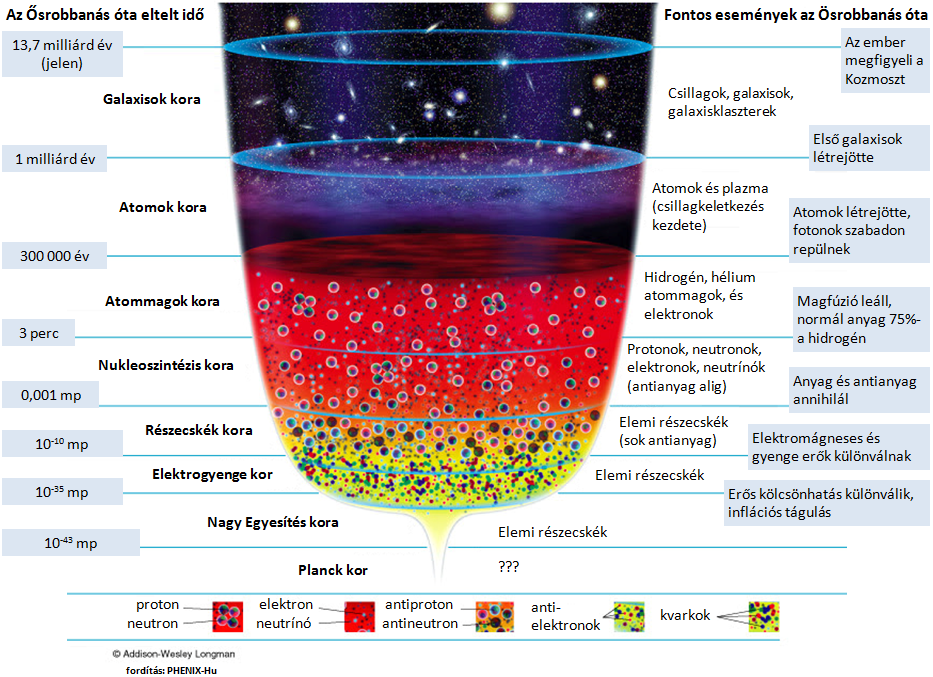
\includegraphics[scale=0.5]{pic/osrobbanas}
\end{frame}

\section{Tökéletes kvarkfolyadék}
\subsection{Kvark-gluon plazma}
\begin{frame}
\frametitle{Kvark-gluon plazma}
\begin{itemize}
\item Az elemi részecskék világának vizsgálata részecskegyorsítókban történik, két legnagyobb LHC és RHIC
\item Hogyan fedezték fel?
\item Kemény folyamatok: nagyenergiás részecskezáporok (jetek) keletkeznek, 2, impulzus megmaradás: ellentétes irányba haladnak
\item Arany-Arany ütközés, nagy centralitás: a jetpár egyik tagja nem jelent meg
\item Próba: Deutérium-arany ütközéseknél semmilyen centralistánál nincs jet-elnyomás
\item Ebből következtettek erősen kölcsönható közeg létrejöttére
\end{itemize}
\end{frame}

\begin{frame}
\begin{center}
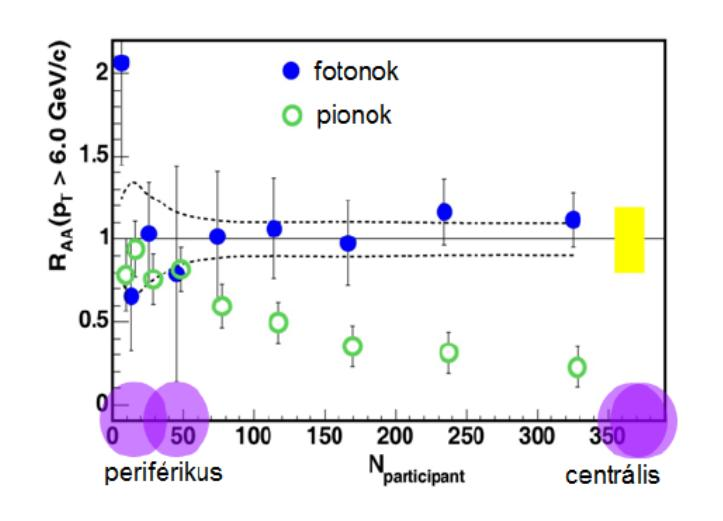
\includegraphics[scale=0.5]{pic/p1}
\end{center}
\end{frame}

\begin{frame}
\frametitle{Kvark-gluon plazma}
\begin{itemize}
\item Az új anyag vizsgálatából kiderült: QGP tökéletes folyadékként viselkedik
\item Tökéletes folyadék: nincs viszkozitás! Ilyen magas hőmérsékleten?
\item AdS/CFT alsó határ viszkozitásra: $\hbar/4\pi$
\item Folyadék: kezdeti eloszlás aszimmetriája megjelenik a detektált részecskék spektrumaiban 
\end{itemize}
\begin{center}
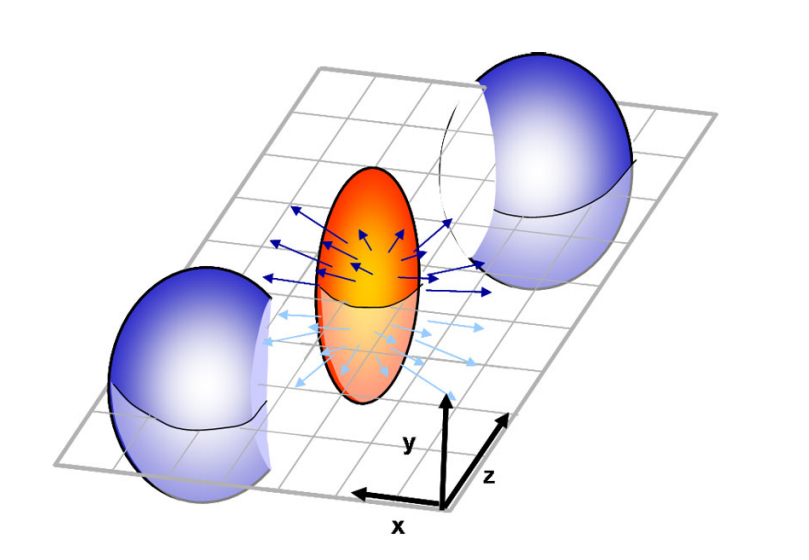
\includegraphics[scale=0.3]{pic/p2}
\end{center}
\end{frame}

\subsection{Hidrodinamika}
\begin{frame}
\frametitle{Hidrodinamika}
\begin{itemize}
\item Folyadékok kollektív viselkedésének leírására: HIDRODINAMIKA
\item Fénysebességhez közeli sebességgel robban a kvarkfolyadék, ezért relativisztikus hidrodinamikát kell alkalmazni (energia-impulzus tenzor általános relativitáselméletből elegánsan kapható)
\end{itemize}
\begin{center}
\begin{equation}
T^{\mu\nu}=(\varepsilon+p)u^\mu u^\nu - p g^{\mu\nu}, \quad  \partial_\mu T^{\mu\nu}=0
\end{equation}
\end{center}
\begin{itemize}
\item Állapotegyenlet: $\varepsilon=\kappa(T)p$
\item Összeütköző atommagok speciális kezdeti eloszlásokat eredményeznek, a kezdeti eloszlásokban megjelenő aszimmetriákat fenti egyenletek szerint fejlődnek az időben
\end{itemize}
\end{frame}

\subsection{Mérhető mennyiségek}
\begin{frame}
\frametitle{Mérhető mennyiségek}
\begin{itemize}
\item A tágulás során a kvarkfolyadék hűl, amikor elér egy bizonyos hőmérsékletet kifagy  (rácsQCD $T_c = 170 MeV$)
\item Kifagyást leírhatjuk:
\begin{center}
\begin{equation}
S(x, p)d^4x=\mathcal{N}n(x)\exp{\bigg(-\frac{p_\mu u^\mu}{T(x)}\bigg)}H(\tau)p_\mu d^3\Sigma_\mu d\tau
\end{equation}
\end{center}

\item A forrásfüggvényt kiintegrálva a teljes térre kapjuk a $p$ impulzusú részecskék számát: $N(p)=\int S(x, p)d^4x$
\item Transzverz síkban a szögfüggő részt Fourier-sorba fejtjük:
\begin{center}
\begin{equation}
N(p_t, \phi)= N(p_t)\bigg(1+\sum_{n=1}^{\infty}\Big[v_n \cos(n\phi)\Big]\bigg)
\end{equation}
\end{center}
\item Legjelentősebb tag $v_2$ (elliptikus folyás), de mások is megjelenhetnek
\end{itemize}
\end{frame}

\begin{frame}
\begin{center}
\begin{figure}[H]
	\centering
    \begin{subfigure}[b]{0.49\textwidth}
    		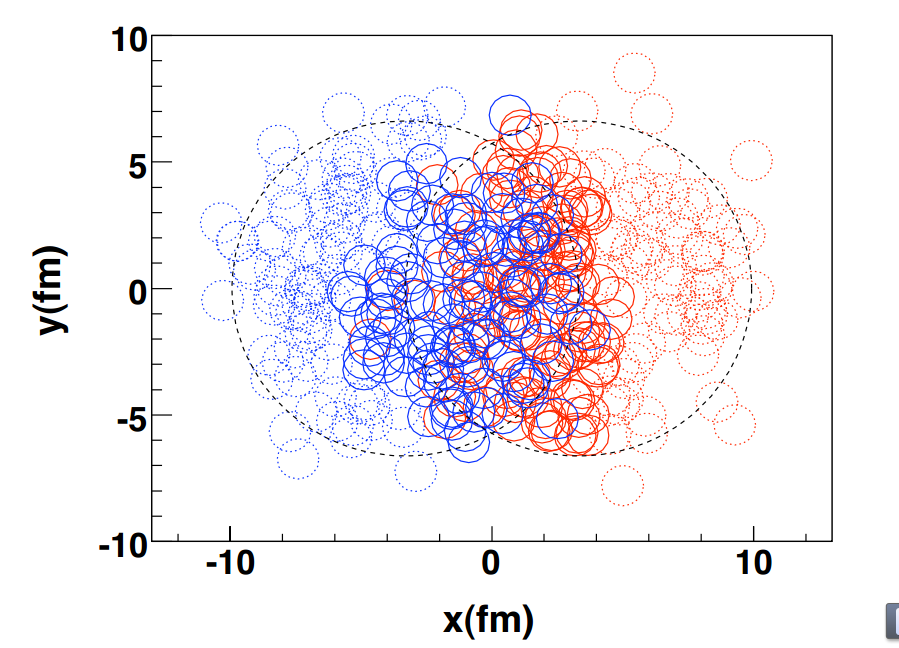
\includegraphics[width=\textwidth]{pic/u1}
	\end{subfigure}
	\begin{subfigure}[b]{0.49\textwidth}
        	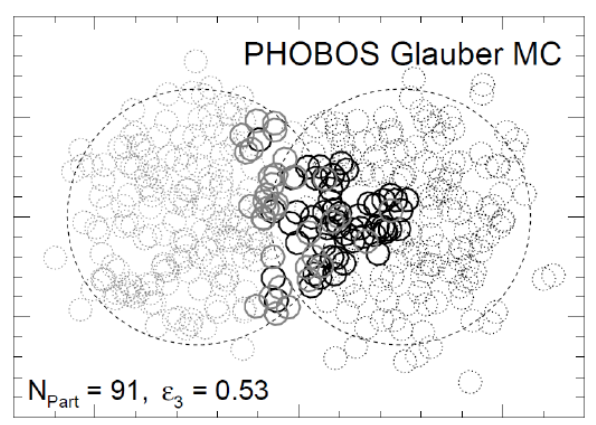
\includegraphics[width=\textwidth]{pic/u2}
	\end{subfigure}
\end{figure}
\end{center}
\end{frame}

\section{A $v_n$ paraméterek mérése}

\subsection{Eseménysík módszer}
\begin{frame}
\frametitle{A $v_n$ paraméterek mérése}
\framesubtitle{Eseménysík módszer}
\begin{itemize}
\item A sorfejtés alapján a paraméterek megkaphatóak: $v_n = \langle cos(n\phi)\rangle$
\item Általában az eseményekre való átlagolást is beleértjük
\item KR: nyalábirányba fölvesszük a z tengelyt, rá merőleges a transzverz sík
\item A z tengely és az ellipszoid legközelebb eső tengelye valamilyen szöget zár be: $\theta_{\rm flow} \approx \langle p_x \rangle/p_{\rm nyalab}$
\item El kell forgatni a KR-et a harmonikusok vizsgálatához! De nagy energián, kicsi a szög, ezért elhanyagoljuk
\end{itemize}
\end{frame}

\begin{frame}
\frametitle{A $v_n$ paraméterek mérése}
\framesubtitle{Eseménysík módszer}
\begin{itemize}
\item Transzverz síkban KR-et a detektorunk kitüntetheti, de ez nem a vizsgált objektumhoz igazodik
\item $v_n$ számolásánál sok eseményre átlagolunk, QGP tetszőlegesen el lehet fordulva, ezért nem tudjuk meghatározni a $v_n$ paramétereket
\item Másodrendű reakciósík: sebességvektorok jelölik ki, $v_2$ kezdőpontja
\item Laborrendszer síkja nem releváns az adatok kiértékelésnél, ezért a másodrendű reakciósíkot tekintjük reakciósíknak
\item Ebben a rendszerben ki meg tudjuk határozni a $v_2$ paramétert
\item Ennek mintájára magasabb rendű reakciósíkok a $v_3$, $v_4$, stb. meghatározására
\end{itemize}
\end{frame}

\begin{frame}
\frametitle{A $v_n$ paraméterek mérése}
\framesubtitle{Eseménysík módszer}
\begin{center}
\begin{figure}
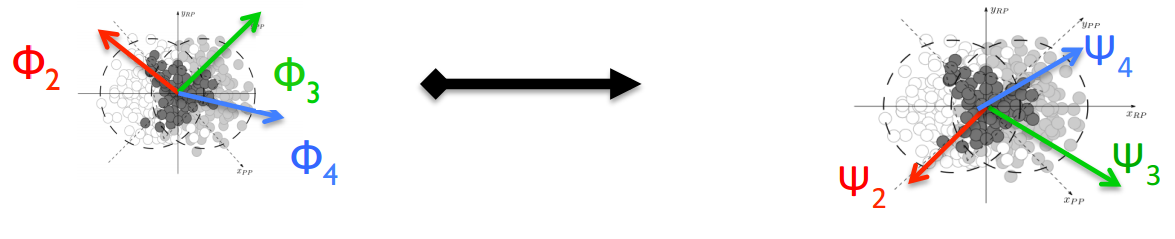
\includegraphics[scale=0.3]{pic/rp}
\end{figure}
\end{center}
\begin{itemize}
\item Nehéz feladat: bázisválasztás
\item Ezek a kvarkfolyadék orientációjához rögzítettek
\item Különböző eseményekre egymásba forgathatjuk
\end{itemize}
\end{frame}

\begin{frame}
\frametitle{A $v_n$ paraméterek mérése}
\framesubtitle{Eseménysík módszer}
\begin{itemize}
\item Tehát a reakciósíkhoz képest mindenik harmonikusnak más a kezdőpontja:
\begin{center}
\begin{equation}
v_n = \langle\cos(n(\phi-\psi_n))\rangle
\end{equation}
\end{center}
\item A $\psi_n$ n-ed rendű reakciósíkot kísérletileg meghatározzuk, ekkor eseménysíknak szoktuk nevezni
\item Az eloszlás n-edik harmonikusának folyási vektorát definiálhatjuk
\begin{center}
\begin{align}
X_n=Q_n \cos(n\psi_n)=\sum_{i}w_i\cos(n\phi) \\
Y_n=Q_n \sin(n\psi_n)=\sum_{i}w_i\sin(n\phi)
\end{align}
\end{center}
\end{itemize}
\end{frame}

\begin{frame}
\frametitle{A $v_n$ paraméterek mérése}
\framesubtitle{Eseménysík módszer}
\begin{itemize}
\item Az n-ed rendű reakciósík meghatározható:
\begin{center}
\begin{equation}
\psi_n = \Bigg(\tan^{-1}\frac{\sum_i w_i \sin(n\phi_i)}{\sum_i w_i \cos(n\phi_i)}\Bigg)\Big/n
\end{equation}
\end{center}
\item Összegzés részecskékre, a $w_i$ súlyok lehetnek például a transzverz impulzus
\item Meghatározzuk a reakciósíkokat, a különböző események esetén egymásba forgatjuk így megkaphatjuk a keresett $v_n$ paramétereket
\item Bármely $n$ harmonikus meghatározható az $m$ reakciósík segítségével amennyiben $n>m$ és $n$ egész számú többszöröse $m$-nek
\end{itemize}
\end{frame}


\begin{frame}
\frametitle{A $v_n$ paraméterek mérése}
\framesubtitle{Eseménysík módszer}
\begin{itemize}
\item A meghatározott $v_n$ értékeben különböző hibák jelennek meg, ezeket korrigálni kell
\item Véges számú részecskét detektálunk ezért szögeloszlást véges pontossággal detektáljuk
\item Ebből adódó hibára lehet korrigálni ha osztunk az eseménysík felbontásával, mert
\begin{center}
\begin{equation}
\langle \cos(n(\phi-\Delta \psi))\rangle = \langle \cos(n\phi)\rangle\langle\cos(n\Delta\psi)\rangle
\end{equation}
\end{center}
\item Tehát erre a hibára korrigálhatunk:
\begin{center}
\begin{equation}
v_n = v_n^{\rm mert}/\langle\cos(km(\psi_m-\psi_r))
\end{equation}
\end{center}
\item $n$ ő akkor $k$ is nő, tehát magasabb rendű harmonikusakat pontatlanabbul mérünk
\end{itemize}
\end{frame}


\subsection{Kumulánsok módszere}

\begin{frame}
\frametitle{A $v_n$ paraméterek mérése}
\framesubtitle{Kumulánsok módszere}
\begin{itemize}
\item Ötlet: keresett paramétereket valahogyan a részecskék korrelációjából határozzuk meg
\item Azimutális (transzverz síkban) sokrészecske korrelációs függvény: $\langle e^{in(\phi_1+...+\phi_k+\phi_{k+1}+...+\phi_{k+l})}\rangle$, átlagolás az összes résecskekombinációra és az eseményekre megy 
\item Kétrészecske korreláció esetén a következőképpen írható:
\begin{center}
\begin{equation}
\langle e^{in(\phi_1-\phi_2)}\rangle=\langle\langle e^{i2(\phi_1-\phi_2)}\rangle\rangle+\langle e^{i2\phi_1}\rangle\langle e^{-i2\phi_2}\rangle
\end{equation}
\end{center}
\item Kifejezés első tagját másodrendű kumulánsnak nevezzük, ez a korrelációt méri, amennyiben nulla részecskék függetlenek
\item Tökéletes detektor esetén a második tag $0$, ekkor a bevezetett korrelációs függvény nulla ha a részecskék közt nincs korreláció
\end{itemize}
\end{frame}

\begin{frame}
\frametitle{A $v_n$ paraméterek mérése}
\framesubtitle{Kumulánsok módszere}
\begin{itemize}
\item Tekintsük a részecskék szögeloszlását:
\begin{center}
\begin{equation}
N(\phi)=\frac{1}{2\pi}\Big[1+\sum_{n}v_n\cos(n(\phi-\psi_n))\Big]
\end{equation}
\end{center}
\item Tökéletes detektort feltételezve felírhatjuk a fenti mennyiségeket:
\begin{center}
\begin{align}
\int_{0}^{\pi}\int_{0}^{2\pi}N(\phi_i)e^{\pm i 2\phi_i }d\phi_id\psi_2 = 0 \\
\int_{0}^{\pi}\int_{0}^{2\pi}\int_{0}^{2\pi}N(\phi_1)N(\phi_2)e^{i 2(\phi_1-\phi_2)}d\phi_1d\phi_2d\psi_2=\frac{v_2^2}{4\pi}
\end{align}
\end{center}
\item Tehát a keresett $v_2$ paraméter a másodrendű kumulánsal megadható $v_2^2=\langle\langle e^{i2(\phi_1-\phi_2)}\rangle\rangle+\langle e^{i2\phi_1}\rangle\langle e^{-i2\phi_2}\rangle$
\end{itemize}
\end{frame}

\begin{frame}
\frametitle{A $v_n$ paraméterek mérése}
\framesubtitle{Kumulánsok módszere}
\begin{itemize}
\item Probléma: nem folyási tagok is adhatnak járulékot a korrelációban (pl. jet)
\item Nem folyási tagok $1/M$-el arányosak, ahol $M$ a detektált részecskék száma
\item Láttuk, hogy folyási tagok $v_n^2$ arányosak
\item Kétrészecske korreláció jó, ha: $v_n\gg 1/\sqrt{M}$
\item Többrészecskés korreláció adhat pontosabb eredményt?
\item Négyrészecske korreláció esetén folyási tagok $v_n^4$
\item Nem folyási tagok pedig $1/M^3$ arányosak
\item Tehát itt $v_n\gg 1/M^{3/4}$, nagy $M$ esetén jelentős különbség
\end{itemize}
\end{frame}

\begin{frame}
\frametitle{A $v_n$ paraméterek mérése}
\framesubtitle{Kumulánsok módszere}
\begin{itemize}
\item Hogy néz ki a négyrészecskés korreláció?
\begin{center}
\begin{align*}
\langle e^{in(\phi_1+\phi_2-\phi_3-\phi_4)}\rangle=\langle\langle e^{in(\phi_1+\phi_2-\phi_3-\phi_4)}\rangle\rangle\\+\langle e^{in(\phi_1-\phi_3)}\rangle\langle e^{in(\phi_2-\phi_4)}\rangle+\langle e^{in(\phi_1-\phi_4)}\rangle\langle e^{in(\phi_2-\phi_3)}\rangle
\end{align*}
\end{center}
\item Ha párosával korreláltak csak a második két tag ad járulékot
\item A kumulánsok előállítására definiáljuk a következő függvényt:
\begin{center}
\begin{align*}
G_n(z)=\prod_{j=1}^{M}\Bigg(1+\frac{ze^{-in\phi_j}+z^*e^{in\phi_j}}{M}\Bigg)
\end{align*}
\end{center}
\end{itemize}
\end{frame}

\begin{frame}
\frametitle{A $v_n$ paraméterek mérése}
\framesubtitle{Kumulánsok módszere}
\begin{itemize}
\item Átlagoljuk az $M$ multiplicitású eseményekre:
\begin{center}
\begin{align*}
\langle G_n(z)\rangle=1+\frac{z}{M}\Big\langle\sum_{j} e^{-in\phi_j}\Big\rangle+\frac{z*}{M}\Big\langle\sum_{j} e^{in\phi_j}\Big\rangle+\frac{z^2}{M}\Big\langle\sum_{j<k} e^{-in(\phi_j-\phi_k)}\Big\rangle\\+...
\end{align*}
\end{center}
\item Sorfejtés
\begin{center}
\begin{align*}
\langle G_n(z)\rangle =1+z\langle e^{-in\phi_1}\rangle +z^{*}\langle e^{in\phi_1}\rangle +\\ \frac{M-1}{M}\Big[\frac{z^2}{2}\langle e^{-in(\phi_1+\phi_2)}\rangle+\frac{z^{*2}}{2}\langle e^{in(\phi_1+\phi_2)}\rangle+\frac{zz^*}{2}\langle e^{in(\phi_1-\phi_2)}\rangle\Big]+...
\end{align*}
\end{center}
\item $z^{*k}z^l$ tagig sorbafejtve épp a $(k+l)$ részecske korrelációt kapjuk
\end{itemize}
\end{frame}

\begin{frame}
\frametitle{A $v_n$ paraméterek mérése}
\framesubtitle{Kumulánsok módszere}
\begin{itemize}
\item Definiáljuk a generátorfüggvényt és fejtsük sorba:
\begin{center}
\begin{align*}
C_n(z)\equiv  M(\langle G_n(z)\rangle^{1/M}+1)=\sum_{k,l}\frac{z^{*k}z^{l}}{k!l!}\langle\langle e^{in(\phi_1+...+\phi_k-...\phi_{k+l})}\rangle\rangle
\end{align*}
\end{center}
\item Tökéletes detektor csak a diagonális elemeket méri, fizikailag csak ezek relevánsak, ezeket jelöljük $c_n\{2k\}=\langle\langle e^{in(\phi_1+...+\phi_k-...\phi_{2k})}\rangle\rangle$
\item Keresett paraméterek felírhatóak: $v_n^2\{2\}=c_n\{2\}$, $v_n^4\{4\}=-c_n\{4\}$
\end{itemize}
\end{frame}

\begin{frame}
\frametitle{A $v_n$ paraméterek mérése}
\framesubtitle{Kumulánsok módszere}
\begin{itemize}
\item Az így kapott paraméterek és a valós paraméterek közti legnagyobb eltérés: nem folyási tagok járuléka
\item $2k$ részecske korrelációban nem folyási tagok járuléka $M^{1-2k}$ nagyságrendű
\item Hiba kicsi legyen: $v_n^{2k}\gg M^{1-2k}$
\item Statisztikus hiba a részecskék véges számából is adódik
\item Hányféleképp választhatunk ki $2k$ eseményt $M$ multiplicitás esetén? (Becslés $M^{2k}N$)
\item A hiba $1/\sqrt{M^{2k}N}$-vel arányos
\item Kísérletben optimális: négyrészecske korreláció
\end{itemize}
\end{frame}

\section{$v_n$ ábrák}
\begin{frame}
\frametitle{Adott kezdőeloszlás, milyen $v_n$ spektrum?}
\begin{center}
\begin{figure}[H]
	\centering
    \begin{subfigure}[b]{0.49\textwidth}
    		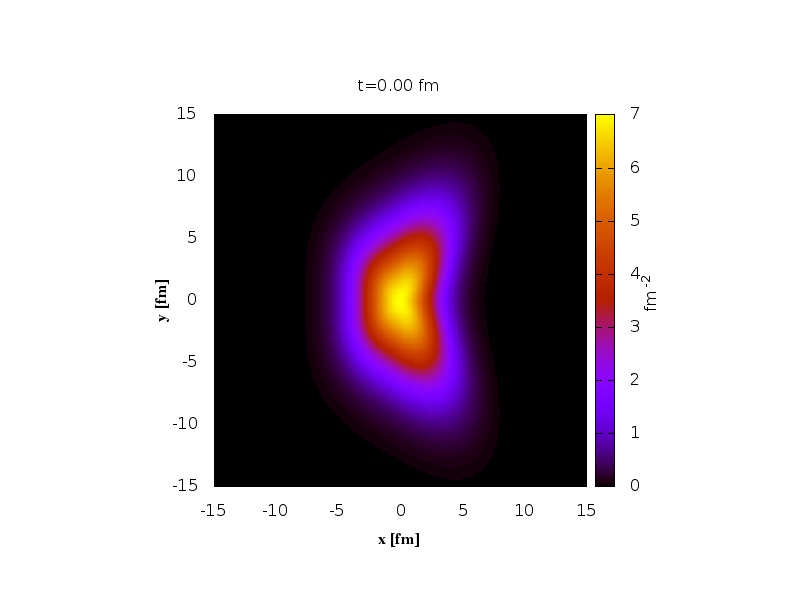
\includegraphics[width=\textwidth]{pic/ini}
	\end{subfigure}
	\begin{subfigure}[b]{0.49\textwidth}
        	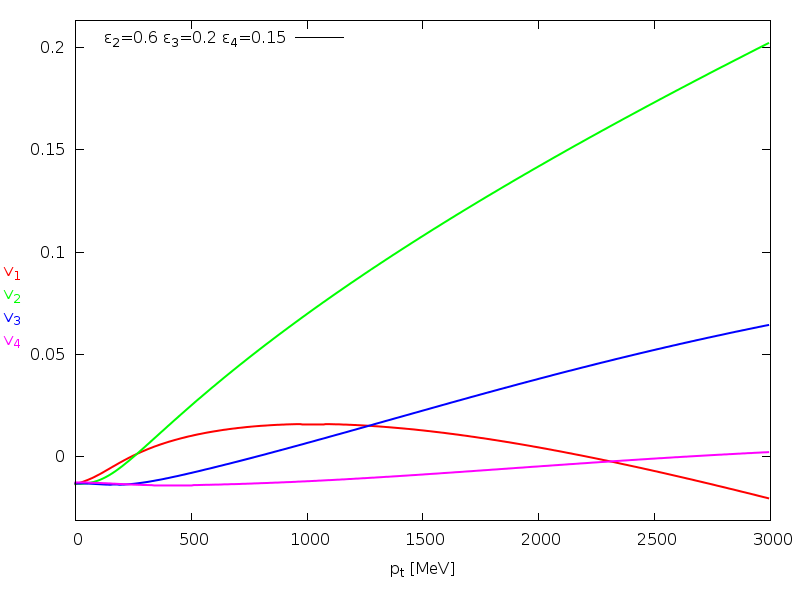
\includegraphics[width=\textwidth]{pic/ini_vn}
	\end{subfigure}
\end{figure}
\end{center}
\end{frame}

\subsection{A $v_2$ különböző centralitás és részecskék esetén}
\begin{frame}
\begin{center}
\begin{figure}[H]
	\centering
    		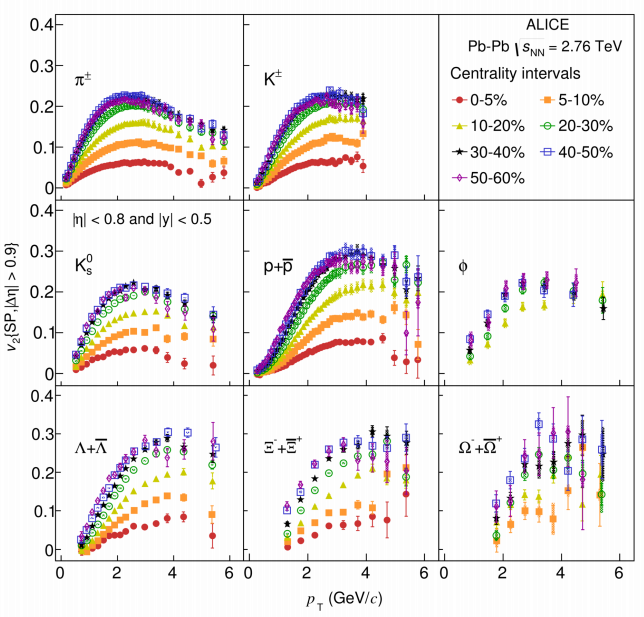
\includegraphics[scale=0.4]{pic/cent}
\end{figure}
\end{center}
\end{frame}


\subsection{Skálaviselkedés}
\begin{frame}
\begin{center}
\begin{figure}[H]
	\centering
    		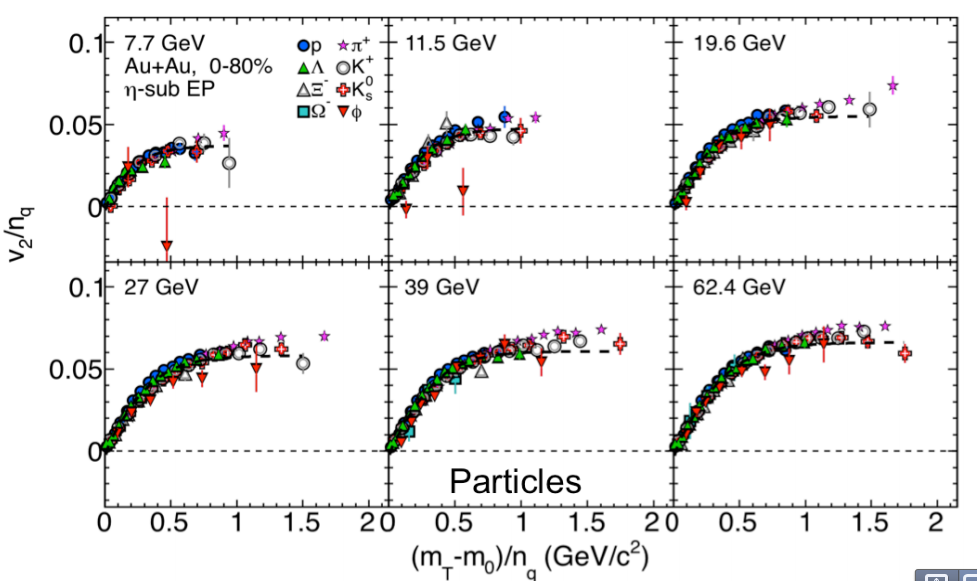
\includegraphics[scale=0.3]{pic/vn_nq}
\end{figure}
\end{center}
\end{frame}

\begin{frame}
\begin{center}
\begin{figure}[H]
	\centering
    		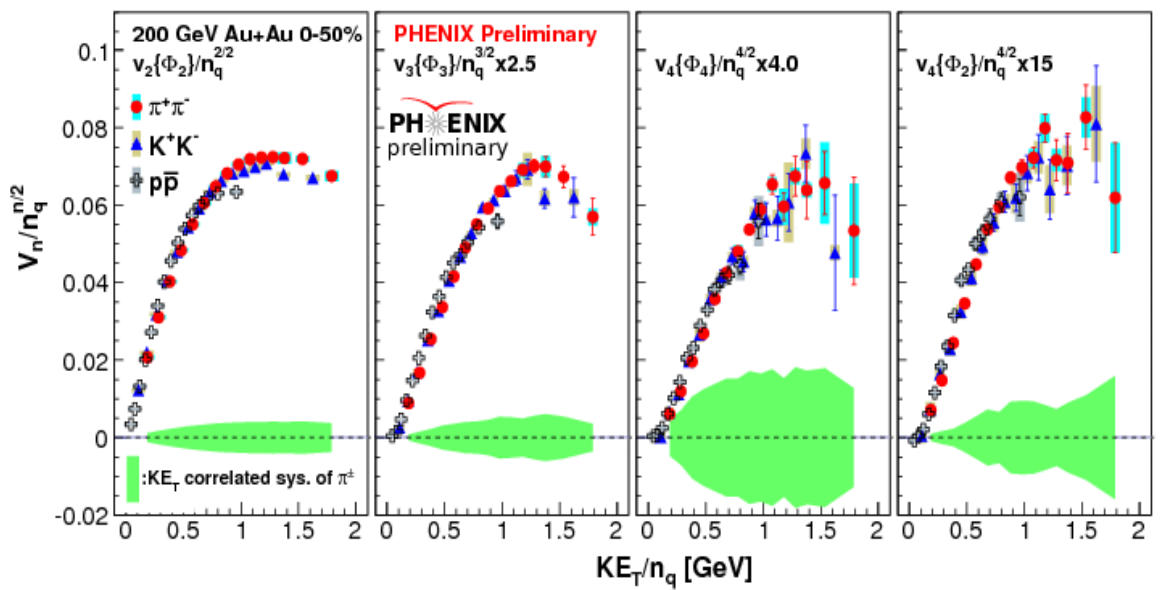
\includegraphics[scale=0.26]{pic/vn_nqn}
\end{figure}
\end{center}
\end{frame}

\begin{frame}
\begin{center}
\begin{figure}[H]
	\centering
    		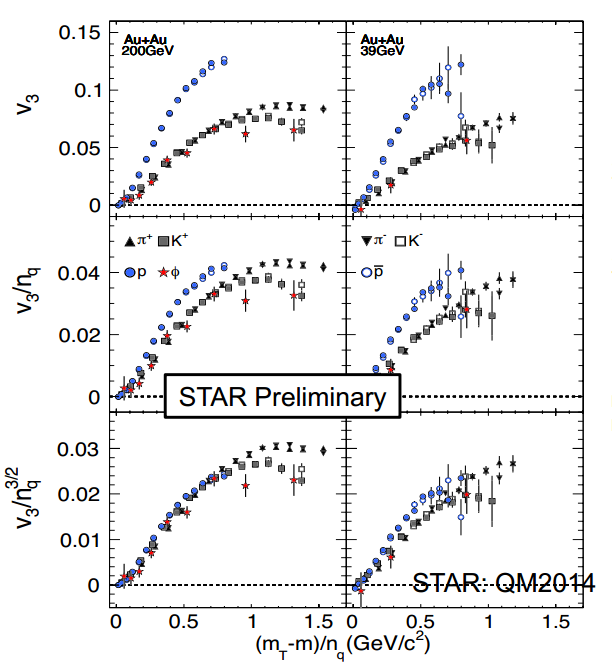
\includegraphics[scale=0.35]{pic/v3_scal}
\end{figure}
\end{center}
\end{frame}

\begin{frame}
\begin{center}
\begin{figure}[H]
	\centering
    		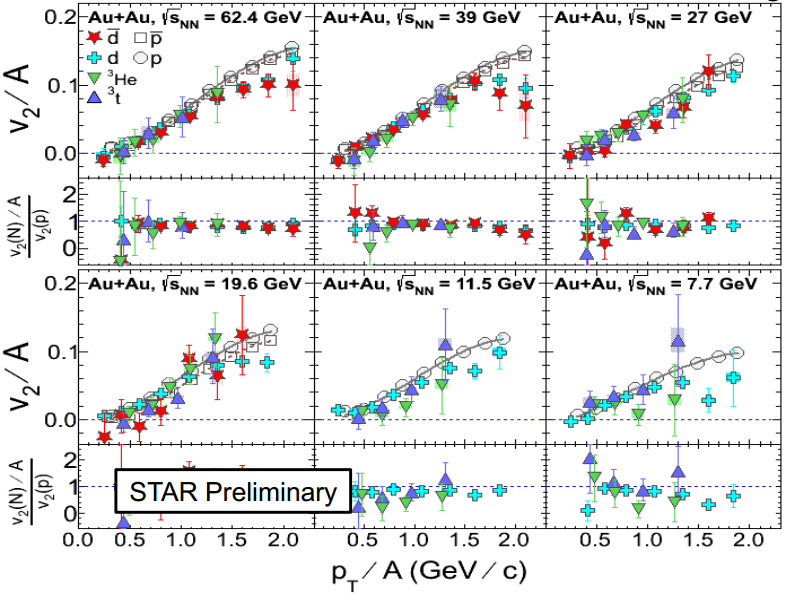
\includegraphics[scale=0.3]{pic/scal_A}
\end{figure}
\end{center}
\end{frame}
\subsection{$J/\psi$ részecske $v_2$ spektruma}
\begin{frame}
\begin{center}
\begin{figure}[H]
	\centering
    		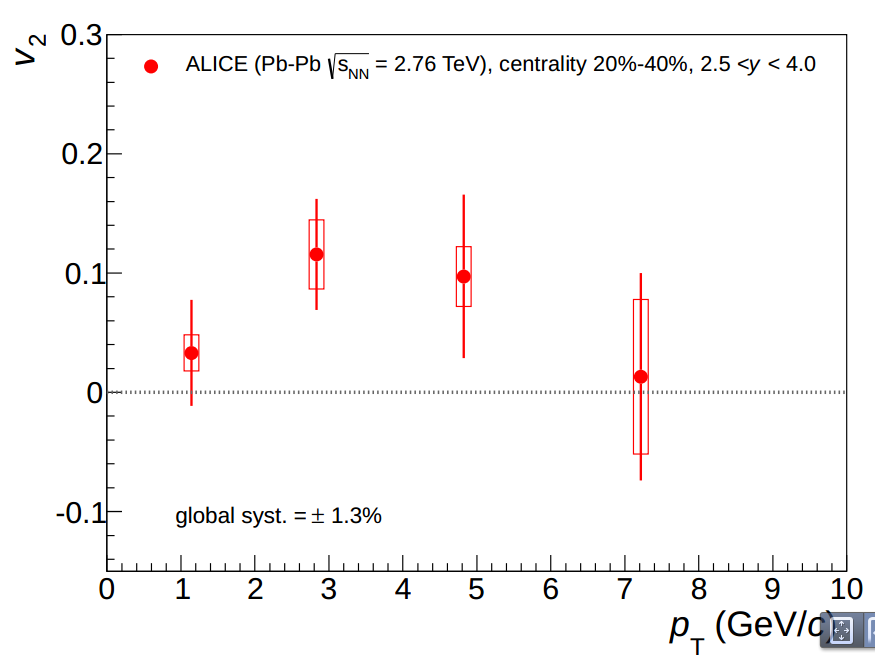
\includegraphics[scale=0.3]{pic/v2_jpsi}
\end{figure}
\end{center}
\end{frame}

\subsection{Direkt fotonok $v_2$ spektruma}
\begin{frame}
\begin{center}
\begin{figure}[H]
	\centering
    		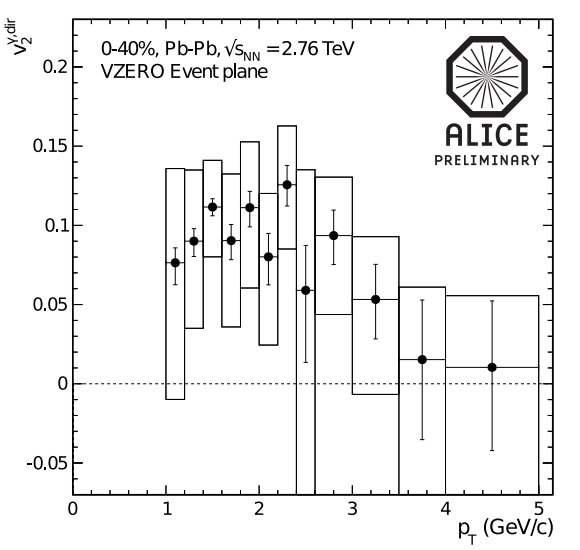
\includegraphics[scale=0.4]{pic/v2_dirphoton}
\end{figure}
\end{center}
\end{frame}


\begin{frame}
\begin{center}
\textbf{Köszönöm a figyelmet!}
\end{center}
\end{frame}


\begin{frame}[noframenumbering]
\frametitle{Hivatkozások}
\end{frame}
\end{document}

